%  !TeX  root  =  user_guide.tex

\section{Road Graph Plugin}\label{sec:roadgraph}

% when the revision of a section has been finalized, 
% comment out the following line:
% \updatedisclaimer


The \toolbtntwo{plugin}{Road Graph} Plugin is a C++ plugin for QGIS, that calculates the shortest path 
between two points on any polyline layer and plots this path over the road network. 

\textbf{Main features}:

\begin{itemize}
\item calculate path, it's length and travel time
\item optimize by length or by travel time
\item export path to a vector layer
\item highlight roads directions (this is slow and used mainly for debug purposes and for the settings 
testing)
\end{itemize}

As a roads layer you can use any polyline vector layer in any QGIS supported format. Two lines with 
a common point are considered connected. Please note, it is required to use layer CRS as project CRS 
while editing roads layer. This is due to the fact that recalculation of the coordinates between 
different CRS introduce some errors that can result in discontinuities, even when 'snapping' is used.

\textbf{In the layer attribute table the following fields can be used}:

\begin{itemize}
\item speed on road section — numeric field;
\item direction — any type, that can be casted to string. Forward and reverse directions are correspond 
to the one-way road, both directions — two-way road.
\end{itemize}

If some fields don't have any value or do not exists — default values are used. You can change defaults 
and some plugin settings in plugin settings dialog.

\minisec{Usage}

After plugin activation you will see additional panel on the left side of the main QGIS window. Now 
make some definitions to the \dialog{road graph plugin settings} dialog in the menu 
\mainmenuopt{Plugins} \arrow \dropmenuopt{Road Graph}. 

\begin{figure}[ht]
    \centering
    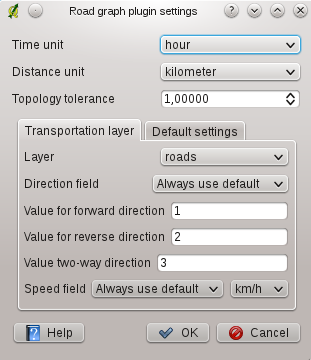
\includegraphics[clip=true, width=5cm]{roadgraph_settings}
    \caption{Define settings for the road graph plugin \nixcaption}\label{fig:roadgraphsettings}
\end{figure}

Select a Start and a Stop point in the road network layer and click on \button{calculate}.

\begin{figure}[ht]
    \centering
    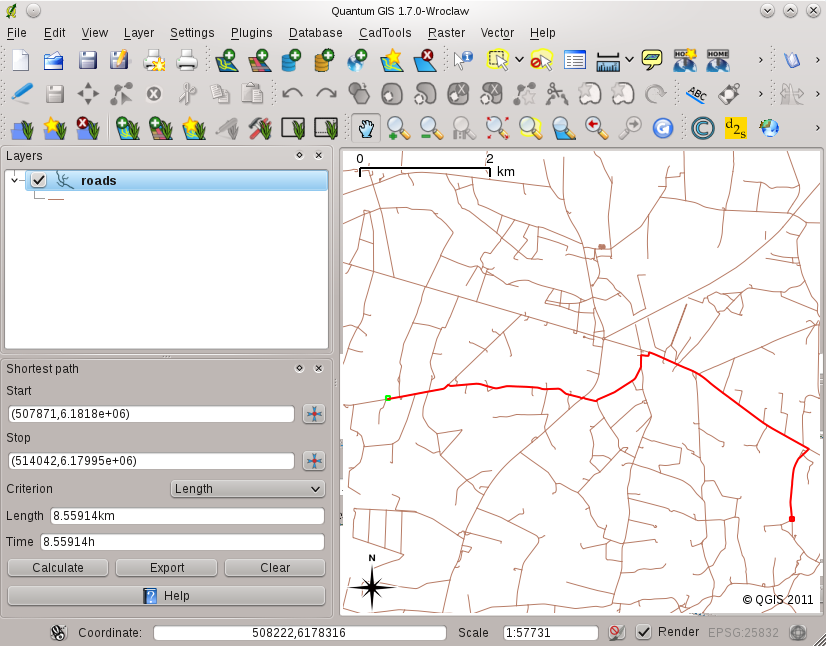
\includegraphics[clip=true, width=12cm]{roadgraph_sample}
    \caption{Road Graph Plugin \nixcaption}\label{fig:roadgraphsample}
\end{figure}

\FloatBarrier
